\documentclass[a4paper]{article}

\usepackage[T1]{fontenc}	
\usepackage{amsmath}
\usepackage{amssymb}
\usepackage{fancyhdr}
\usepackage{booktabs}
\usepackage{graphicx}
\usepackage{float}
\usepackage{algpseudocode}
\usepackage{algorithm}
\usepackage[margin=1in]{geometry}

\pagestyle{fancy}
\rhead{Home Assignment 3}
\lhead{Noah Hansson \& Kristoffer Nordström}

\title{Home Assignment 3 - FMSN50}
\author{Kristoffer Nordström, Noah Hansson}\author{Kristoffer Nordström \\ kr8245no-s@student.lu.se \and  Noah Hansson \\ no3822ha-s@student.lu.se}
\date{\today}


\setlength{\parskip}{0.7em}
\setlength{\parindent}{0pt}
\setlength{\floatsep}{6pt plus 1.0pt minus 2.0pt}
\setlength{\textfloatsep}{10pt plus 1.0pt minus 2.0pt}

\begin{document}
\maketitle
\newpage

\section*{Coal mine disasters - Constructing a complex MCMC algorithm}


\subsection*{a) Posterior probabilities}
We are interested in sampling from the posterior distribution $f(\lambda, \theta, t | \tau)$ using a hybrid MCMC algorithm. To do this, we must first find the marginal posterior distributions:
\begin{itemize}
    \item $f(\theta | \tau, \lambda, t)$
    \item $f(t | \tau, \lambda, \theta)$
    \item $f(\lambda | \tau, \theta, t)$
\end{itemize}

To do this we begin by reducing the dimension of the posterior using the Bayes' theorem and the chain rule, giving us:
\begin{equation}
    f(\lambda, \theta, t | \tau) \propto f(\tau|\lambda, \theta, t)f(\lambda, \theta,t) = f(\tau|\lambda,t)f(t)f(\theta)f(\lambda|\theta)
\end{equation}
From this, we can find the marginal posterior distributions up to a normalizing constant:
\begin{equation}
    \begin{cases}
        f(\theta | \tau, \lambda, t) \propto f(\theta)f(\lambda|\theta) \\
        f(t | \tau, \lambda, \theta) \propto f(t)f(\tau|\lambda,t) \\
        f(\lambda | \tau, \theta, t) \propto f(\lambda|\theta)f(\tau|\lambda,\theta)
    \end{cases}
\end{equation}

From these marginal distributions we can attempt to find a general distribution to sample the variables. For $\lambda$ this gives us:
\begin{equation}
    \begin{gathered}
        f(\lambda | \tau, \theta, t) \propto f(\lambda|\theta)f(\tau|\lambda,\theta) = \\ = \theta^2\lambda\exp(-\theta\lambda-\sum_{i=1}^d(t_{i+1}-t_i))\prod_{t=1}^d\lambda_i^{n_i(\tau)}
    \end{gathered}
\end{equation}
Since lambda is a vector of intensities $\lambda_i$ we can sample each individual lambda as 
\begin{equation}
    f(\lambda_i|\theta)f(\tau|\lambda_i,t) = \theta^2\lambda_i^{n_i(\tau)+1}\exp(-\lambda_i(\theta + (t_{i+1}-t_i)))
\end{equation}
From this expression we can conclude that the marginal posterior for $\lambda$ is gamma distributed such that:
\begin{equation}
    \lambda_i \sim \Gamma(2+n_i(\tau), \theta + (t_{i+1} - t_i))
\end{equation}

Similarly, for $\theta$:
\begin{equation}
    \begin{gathered}
        f(\theta|\tau, \lambda, t) \propto f(\theta)f(\lambda|\theta) = f(\theta)\prod_{i=1}^d f(\lambda_i|\theta)= \\
        = \Psi^2\theta\exp(-\theta\Psi)\prod_{i=1}^d(\theta^2\lambda_i\exp(-\lambda_i\theta)) = \\
        = \Psi^2\theta^{2d+1}\exp(-\theta(\Psi+\sum_{i=1}^d\lambda_i))\prod_{i=1}^d\lambda_i
    \end{gathered}
\end{equation}
Here we can conclude that the marginal posterior for $\theta$ is gamma distributed such that:
\begin{equation}
    \theta \sim \Gamma(2+2d, \Psi+\sum_{i=1}^d\lambda_i)
\end{equation}

Unfortunately the marginal distribution of $t$ cannot be sampled from a known distribution. This is why we need a hybrid MCMC sampler to sample from the posterior. The hybrid sampler can use the Gibbs algorithm for $\theta$ and $\lambda$ since they can be sampled from, but we will need to use the Metropolis Hastings algorithm for $t$.


\subsection*{b) The hybrid MCMC algorithm}

To sample from $f(\lambda, \theta, t | \tau)$ we need to construct a hybrid MCMC sampler using both the Gibbs sampler and the Metropolis-Hastings algorithm. A pseudocode outline of the algorithm is presented below:

\begin{algorithm}
    \caption{Pseudocode of the hybrid MCMC sampler where M is the number of samples plus burn-in samples, and d is the number of breakpoints.}
    \begin{algorithmic}
        \State Initiate $t_1$ evenly spaced in the interval [1658,1980]
        \State Sample $\theta_1 \sim \Gamma(2,\Psi)$
        \State Sample $\lambda_1 \sim \Gamma(2,\theta_1)$
        \For{$k = 1:M$}
        \State Sample $\theta_{k+1}$ from $f(\theta|\tau, \lambda_k, t_k)$
        \State Sample $\lambda_{k+1}$ from $f(\lambda|\tau, \theta_{k+1}, t_k)$
        \For{$i = 1:d$}
        \State Propose $t_{k+1}^i$ from a random walk proposal
        \State Accept or reject $t_{k+1}^i$
        \EndFor
        \EndFor
    \end{algorithmic}
\end{algorithm}

Since we cannot find a known distribution for $t$ we instead need to find a proposal kernel $r(z|x)$ that results in a proper MH sampler. We aim to use a symmtric proposal kernel for $t$, which means that $r(z|x) = r(x|z)$. In this case we use the random walk proposal:

\begin{equation}
    \label{eq:proposal_kernel}
    \begin{gathered}
        t_i^\star = t_i + \epsilon \\
        \text{with} \\
        \epsilon \sim U(-R,R) \\
        \text{and} \\
        R = \rho(t_{i+1}-t_{i-1})
    \end{gathered}
\end{equation}

By using a symmetric proposal we can easily calculate the acceptance probability for the MH step. The MH acceptance probability is calculated as follows:
\begin{equation}
    \alpha(x,z) = 1 \wedge \frac{f(z)r(x|z)}{f(x)f(z|x)}
\end{equation}
Which when using a symmetric proposal kernel simplifies to
\begin{equation}
    \alpha(x,z) = 1 \wedge \frac{f(z)}{f(x)}
\end{equation}
Which means that for the random walk proposal of $t$ we get the acceptance probability as
\begin{equation}
    \alpha(x,z) = 1 \wedge \frac{f(t^\star | \tau, \lambda, \theta)}{f(t | \tau, \lambda, \theta)} = 1 \wedge \frac{f(t^\star)f(\tau|\lambda,t^\star)}{f(t)f(\tau|\lambda,t)}
\end{equation}
which means that we can calculate the acceptance probability from known proability density functions.
\subsection*{c) Results for different amounts of break points}

We proceed by running the simulation for different amount of breakpoints to how the behaviour of the chain varies. The results are plotted in figure \ref{fig:num_breakpoints_results}.

\begin{figure}[H]
    \centering
    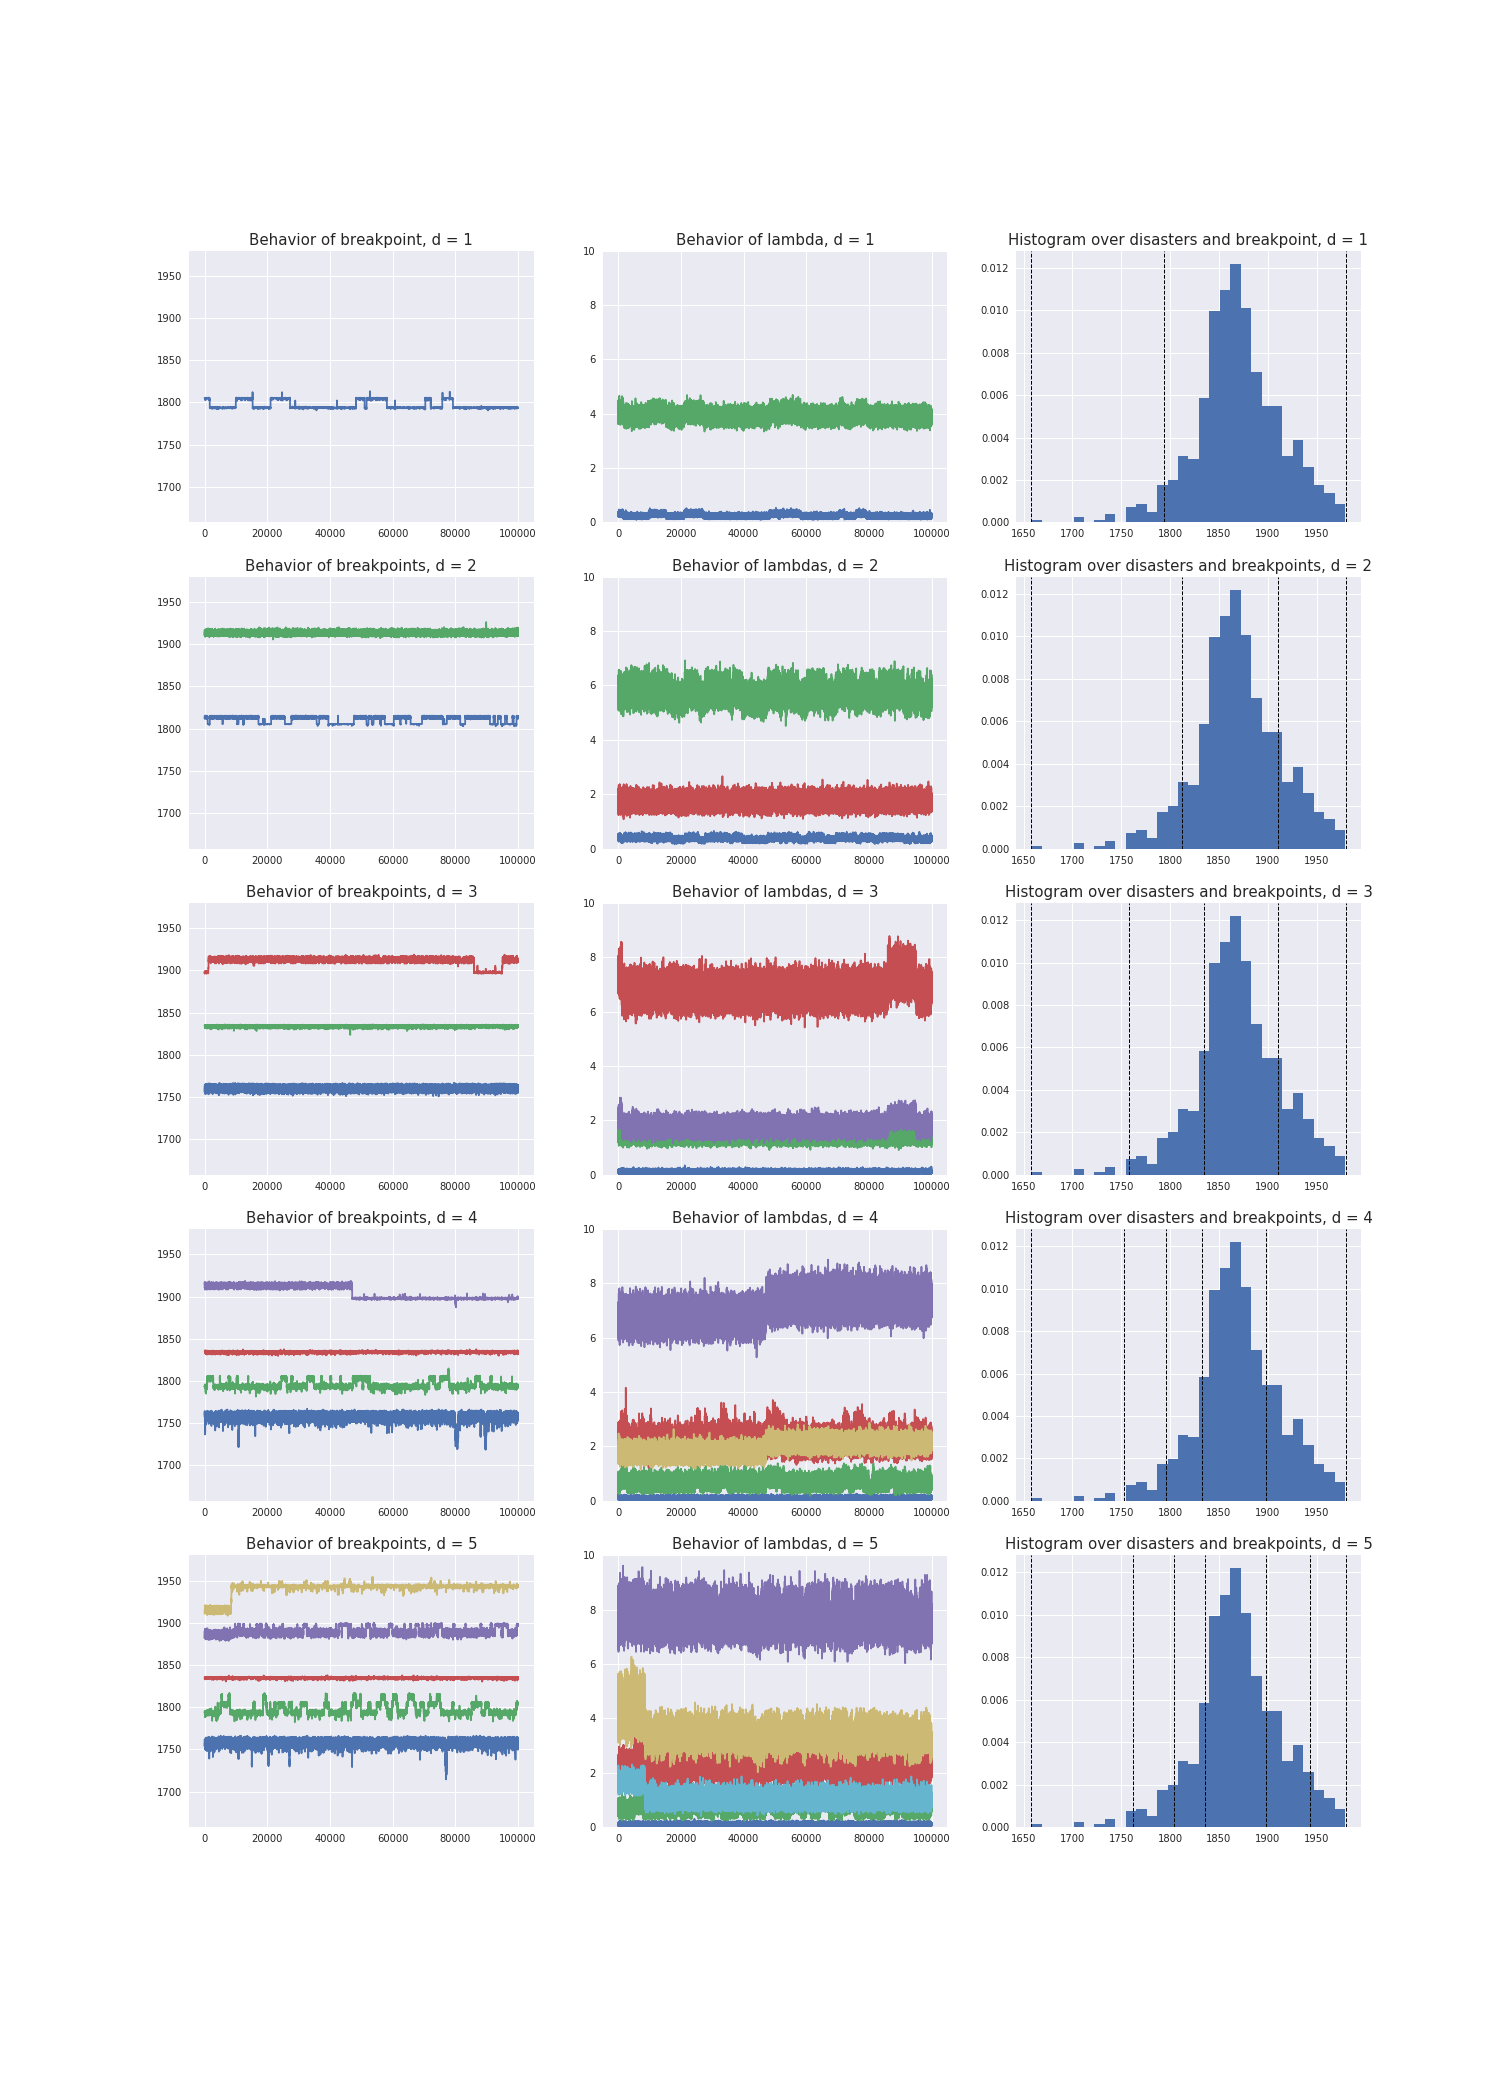
\includegraphics[width = 1.0\textwidth]{images/chain_behavior.png} 
    \caption{Behaviour of the Markov Chain for the breakpoints and intensities, as well as the final breakpoints, for 1 to 4 breakpoints. The sample size is 10 000 with a burn in size of 1000 samples. $\Psi$ is set to $20$ and $\rho$ is set to $0.025$. The acceptance rates are presented in table \ref{tab:acceptance_rates}}
    \label{fig:num_breakpoints_results}
\end{figure}

\begin{table}
    \centering
    \caption{Acceptance probabilities for each simulation presented in figure \ref{fig:num_breakpoints_results}}
    \label{tab:acceptance_rates}
    \begin{tabular}{lrrrrr}
\toprule
Number of breakpoints &    d = 1 &     d = 2 &     d = 3 &     d = 4 &     d = 5 \\
\midrule
      Acceptance rate &  0.04927 &  0.213045 &  0.264037 &  0.345295 &  0.388494 \\
\bottomrule
\end{tabular}

\end{table}

As seen in figure \ref{fig:num_breakpoints_results} the algorithm manages to converge rather fast towards the true values. As the number of breakpoints increase, we note that the chains start to jump more. This is due to the strong dependencies between the breakpoints. If one breakpoint struggles to converge or has a large variance, it effects the variance and sampling of the other breakpoints. As the number of breakpoints increase the variance and amount of jumps also increases. We also note from table \ref{tab:acceptance_rates} that as the amount of breakpoints increases, the acceptance rates go up. This is probably related to the fact that as the amount of breakpoints increases, the step length for the random walk proposal decreases. The acceptance rates as a function of step length will be explored further in section e).

\subsection*{d) Dependance on hyperparameter $\Psi$}
When sampling $\lambda$ the prior distribution is  $\lambda \sim \Gamma(2,\theta)$, where $\theta \sim \Gamma(2,\Psi)$. The parameter $\Psi$ is a hyperparameter specified when initiating the algorithm. Here we will try to estimate the parameters $\theta$ and $\lambda$ for different choices of $\Psi$ and see how the parameter choice effects the process parameters. The results are presented in figure \ref{fig:different_psi}.

\begin{figure}[H]
    \centering
    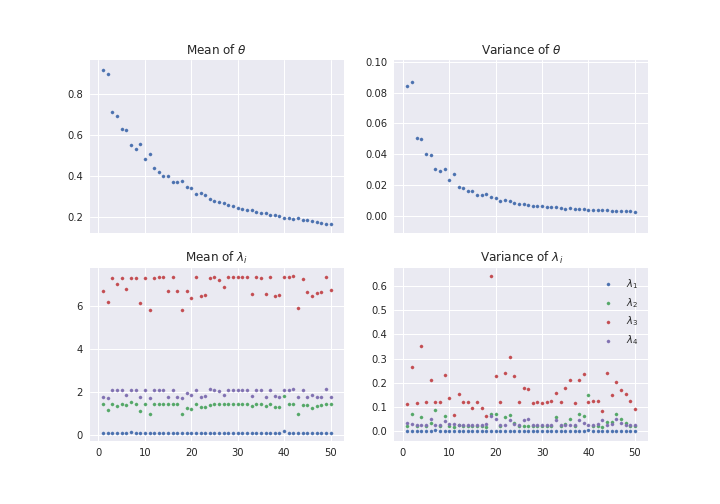
\includegraphics[width = 1.0\textwidth]{images/psi.png} 
    \caption{Mean and variance of $\theta$ and $\lambda$ as a function of hyperparameter $\Psi$. Here we are simulating $10 000$ samples with 3 breakpoints and $\rho = 0.025$}
    \label{fig:different_psi}
\end{figure}

Here we can see that as $\Psi$ increases $\theta$ decreases. However, this does not seem to have a significant effect on $\lambda$, as the mean and variance seems rather constant.

\subsection*{e) Dependance on proposal parameter $\rho$}
Another parameter specified when initiating the algorithm is the parameter $\rho$ which is used in the proposal kernel for $t$ (see equation (\ref{eq:proposal_kernel})). The parameter can be interpreted as a coefficient in the step length of the random walk proposal. If $\rho$ is large the proposal on average takes larger steps compared to when $\rho$ is small. A large $\rho$ results in faster movement but with smaller acceptance rates. A small $\rho$ gives slow movement but higher acceptance rate. To measure the mixing we look at the ACF for the sampled breakpoints. Fast mixing implies that the ACF decreases fast, while slow mixing gives autocorrelation for many iterations. As we can see in figure \ref{fig:acf} the ACF declines the fastest when $\rho$ is around 0.025 - 0.0325, for this $\rho$ we get an acceptance factor of approximately 30\% as seen in figure \ref{fig:accept_rho}, this is in line with the general recommendation.

For the following attempts we use $10 000$ samples a burn in of $1000$ and $\Psi = 20$.

\begin{figure}[H]
    \centering
    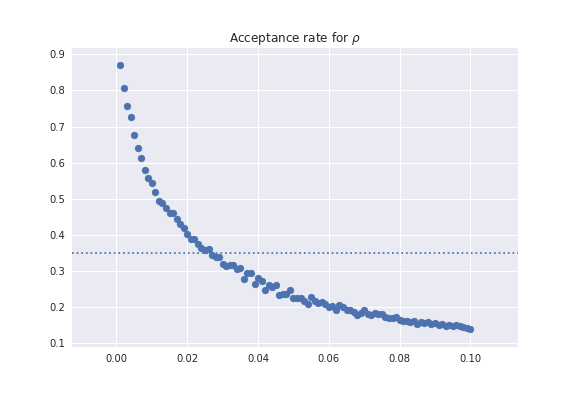
\includegraphics[width = 1.0\textwidth]{images/accept_rho.png} 
    \caption{Acceptance rate for $\rho$ between 0.001 and 0.1}
    \label{fig:accept_rho}
\end{figure}

\begin{figure}[H]
    \centering
    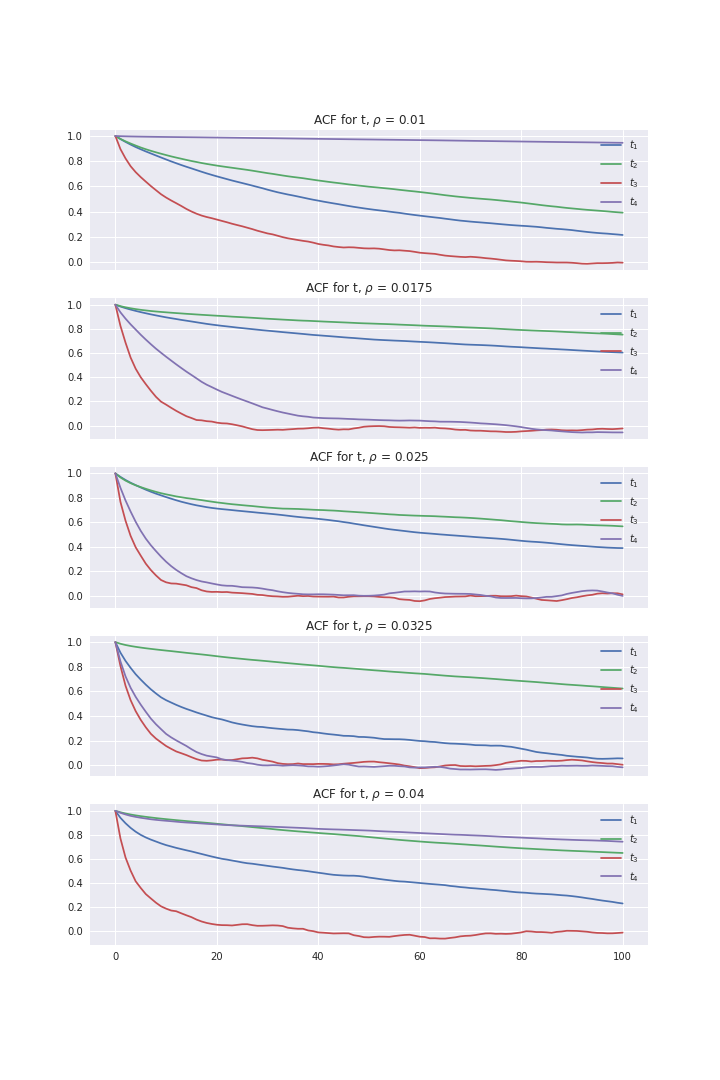
\includegraphics[width = 1.0\textwidth]{images/ACF.png} 
    \caption{ACF for the breakpoints for different timesteps and different values of $\rho$}
    \label{fig:acf}
\end{figure}

The mean and variance for $\theta$ and $\rho$ was calculated for simulations for $\rho$ between $0.01$ and $0.1$. The simulations was made with the same settings as above. As we can see in figure \ref{fig:thetha_rho} both $\theta$ and $\lambda$ is mostly unaffected by the change of $/rho$. One can see a bit more variance in $\lambda$ when $\rho$ is larger, but this is quite reasonable due to the fact that a larger $\rho$ results in bigger jumps of $t_i$.

\begin{figure}[H]
    \centering
    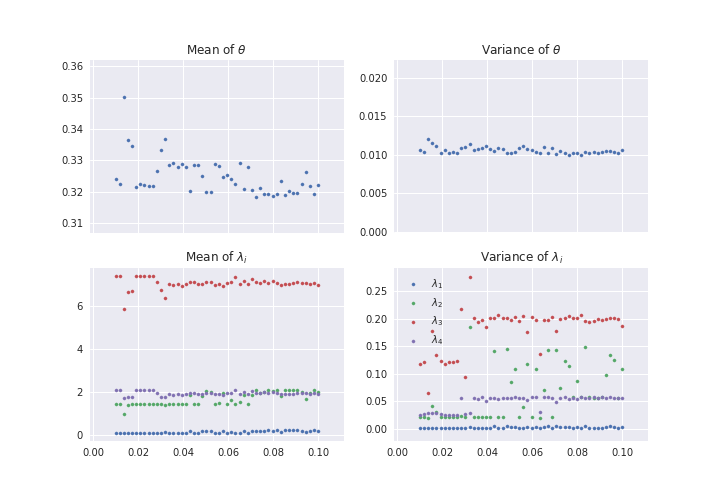
\includegraphics[width = 1.0\textwidth]{images/rhos_theta.png}
    \caption{How $\theta$ and $\lambda$ behave for $\rho$ between 0.001 and 0.1}
    \label{fig:thetha_rho}
\end{figure}

\newpage

\section{Parametric bootstrap for the 100-year Atlantic wave}

\subsection*{a) Finding the inverse of the Gumbal distribution}

The Gumbal distribution has the following cumulative distribution function

\begin{equation}
    F(x; \mu, \beta) = \exp\left(-\exp\left(-\frac{x-\mu}{\beta}\right)\right), \quad x \in \mathbb{R}
    \label{eq:gumbel}
\end{equation}

For a uniformly distributed variable $u \in [0,1]$ we calculate the inverse as:

\begin{equation}
    \label{eq:inv_gumbel}
    \begin{gathered}
        F(F^{-1}(u;\mu, \beta)) = u \iff \exp(-\exp(\frac{F^{-1}(u;\mu,\beta)-\mu}{\beta})) = u \\
        \iff \\
        F^{-1}(u; \mu, \beta) = \mu - \beta*\ln(-\ln(u)), \quad u\in [0,1]
    \end{gathered}
\end{equation}


\subsection*{b) Parametric bootstrap of parameter estimates}

Given measurements assumed to belong to a distribution we are interested of finding a confidence interval of the estimated parameters. In this case, we are given measurements of wave heights that we assume are distributed from a Gumbel distribution. To find the confidence interval we then use a parametric bootstrap to find the variance of the parameters. To get a confidence interval the bootstrap is conducted as follows:

\begin{algorithm}
    \caption{Pseudocode of the paremetric bootstrap of parameter estimates}
    \begin{algorithmic}
        \State Estimate parameters $\hat{\mu}$ and $\hat{\beta}$ from the given data
        \For{i = 1:N}
        \State Simulate bootstrap $B_i \sim Gumbel(\hat{\mu}, \hat{\beta})$
        \State Estimate parameters $\mu_{B_i}$ and $\beta_{B_i}$
        \State Find bootstrap error $\Delta_i = [\hat{\mu_{B_i}}, \hat{\beta_{B_i}}] - [\hat{\mu}, \hat{\beta}]$
        \EndFor
        \State Find $0.025$ and $0.975$ quantiles of $\Delta$
        \State Create confidence intervals using quantiles of $\Delta$ and estimated parameters $\hat{\mu}$ and $\hat{\beta}$
    \end{algorithmic}
\end{algorithm}

The resulting confidence interval for the parameters can be seen in table \ref{tab:parameters} and in figure \ref{fig:bootstrap_res}.

\begin{table}[H]
    \centering
    \caption{Estimated parameters with 95\% bootstrapped confidence intervals.}
    \label{tab:parameters}
    \begin{tabular}{lrrr}
\toprule
Parameter &  Estimate &  95\% Upper bound &  95\% Lower bound \\
\midrule
  $\beta$ &     1.486 &             1.579 &             1.390 \\
    $\mu$ &     4.148 &             4.277 &             4.022 \\
\bottomrule
\end{tabular}

\end{table}

\subsection*{c) Parametric bootstrap of the highest wave}

To calculate the one sided parametric bootstrapped 95\% confidence interval for the 100-year we begin by constructing bootstraps as in b), and then estimate the 100-year wave for each set of bootstrap parameter estimates.

The resulting confidence interval for the 100-year wave can be seen in table \ref{tab:bigwave} and in figure \ref{fig:bootstrap_res}.

\begin{algorithm}
    \caption{Pseudocode of the paremetric bootstrap the 100-year wave. T = 3*14*100 = 4200}
    \begin{algorithmic}
        \State Estimate parameters $\hat{\mu}$ and $\hat{\beta}$ from the given data
        \For{i = 1:N}
        \State Simulate bootstrap $B_i \sim Gumbel(\hat{\mu}, \hat{\beta})$
        \State Estimate parameters $\mu_{B_i}$ and $\beta_{B_i}$
        \State Evaluate $F(1-1/T; \hat{\mu_{B_i}}, \hat{\beta_{B_i}})$
        \State Find bootstrap error $\Delta_i = F(1-1/T; \hat{\mu}, \hat{\beta}) - F(1-1/T; \hat{\mu_{B_i}}, \hat{\beta_{B_i}})$
        \EndFor
        \State Find $0.95$ quantile of $\Delta$
        \State Create one-sided confidence interval using the quantile of $\Delta$ and the estimate $F(1-1/T; \hat{\mu}, \hat{\beta})$
    \end{algorithmic}
\end{algorithm}

\begin{table}[H]
    \centering
    \caption{Estimated mean of the 100-year way and bootstrapped one sided 95\% confidence interaval}
    \label{tab:bigwave}
    \begin{tabular}{lrr}
\toprule
     Parameter &    Mean &  95\% Upper bound \\
\midrule
 100-year wave &  16.527 &            17.235 \\
\bottomrule
\end{tabular}

\end{table}

\begin{figure}[H]
    \centering
    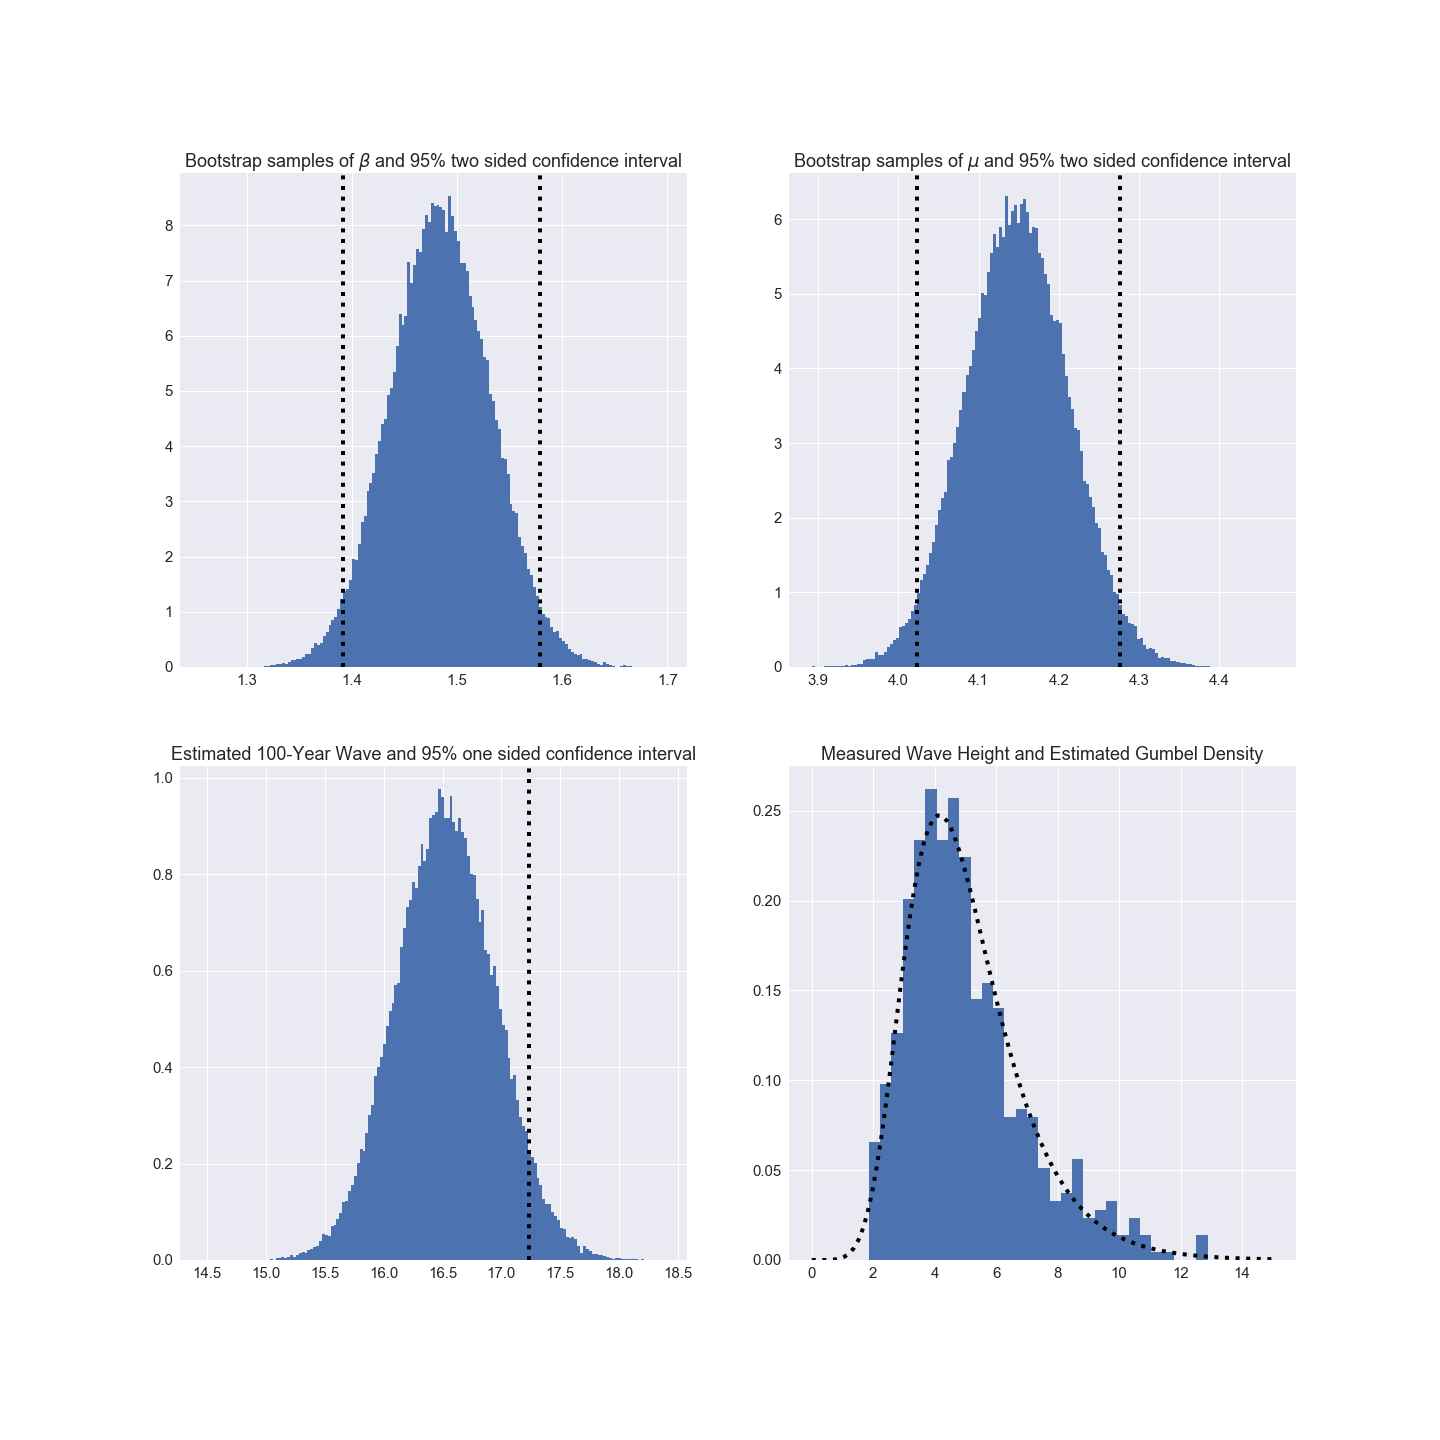
\includegraphics[width = 1.0\textwidth]{images/results_bootstrap.png}
    \caption{Densities over bootstrapped parameters $\beta$ and $\mu$, }
    \label{fig:bootstrap_res}
\end{figure}
\end{document}